\section{March 10}
Recall that in the last lecture, we derived the following form for the Green's function equation in momentum
space:
\[
	G(t, \mathbf{r}) = \int \frac{d^{4}k}{(2\pi)^{4}} \frac{ e^{i k\cdot x}}{(k^{0})^2 - |\mathbf{k}|^2}
\]
The denominator is troubling, because it implies that the integrand blows up to infinity when \( k^{0} =
\pm |\mathbf{k}| \), so we need to evaluate this integral using complex analysis. We will introduce all the
tools necessary for complex analysis necessary in class, so there's no need to look for outside sources.
However, for a full treatment of complex analysis (highly recommended!) you should go take a full course on
it -- there's just no way to do it justice in 3 lectures of time. With that said, let's try our best to
illustrate the main components we'll need from complex analysis.   

\subsection{Complex Analysis}
To start, let's consider the basic complex plane:
\begin{center}
	\begin{tikzpicture}
		\draw (-3, 0) -- (3, 0) node[right] {\( x = \Re(z)\)}; 
		\draw (0, -3) -- (0, 3) node[above] {\( y = \Im(z) \)};
		\draw[red!80!white, -stealth] (0, 0) -- (2, 1) node[above right] {\( z = x + iy \)};
	\end{tikzpicture}
\end{center}
A complex number can always be decomposed into its real and imaginary component, in the form \( z = x + iy
\). This can be represented in the complex plane as a point \( (x,y) \), so in this sense you can think of
the complex plane as an \textit{analogue} of \( \R^2 \), but there are key differences, as we shall see in
the coming lectures. 
We can also define the complex conjugate of \( z \) as \( z^{*} = x - iy \), where we basically flip the
imaginary component. Now, motivated by this real-imaginary decomposition, we can define a complex function \(
f : \C \to \C \) as a map that takes one complex number \( (x, y) \) and transforms it into another complex
number, written as:
\[
	f(x, y) = u(x, y) + iv(x, y)
\]
So just like we can separate complex numbers, we can separate functions too. Now, if we are to consider the
derivative of \( f(z) \):
\[
	\dv{f}{z}\eval_{z_0}
\]
This is not always uniquely defined in the complex plane. The reason is because in principle there are many
different ways that you can approach \( z_0 \) in the complex plane -- from the left, right, above, etc.. So,
in order for the derivative to exist, what needs to be shown is that in \textit{all} the ways we can approach \(
z_0\), the quantity:
\[
	\lim_{\Delta z \to 0 } \frac{f(z_0 + \Delta z) - f(z_0)}{\Delta z}
\]
exists and is the same, only then can we conclude that \( f(z) \) is differentiable at \( z_0 \). Because
this is true for any \( dz \) chosen, one necessary condition for differentiability is then that the
derivative is the same when \( dz = dx \) and \( dz = i dy \). If these are equal, this means:
\begin{align*}
	\pdv{f}{x} &= \frac{1}{i}\pdv{f}{y} \\ 
	\pdv{u}{x} + i\pdv{v}{x} &= \frac{1}{i}\left( \pdv{u}{y} + i \pdv{v}{y} \right) = -i \pdv{u}{y} +
	\pdv{v}{y}
\end{align*}
Comparing the real and imaginary parts, we get the system of equations: 
\[
	\pdv{u}{x} = \pdv{v}{y} \quad \pdv{v}{x} = -\pdv{u}{y}
\]
These are canonically called the \textbf{Cauchy-Riemann Conditions}. Note also that we can express this in
terms of \( \partial_{z^{*}}f \). Recall that \( z = x + iy \) and \( z^{*} = x - iy \), so therefore:
\begin{align*}
	\pdv{z} &= \pdv{x}{z} \pdv{x} + \pdv{y}{z} \pdv{y} = \frac{1}{2}\pdv{x} + \frac{1}{2i}\pdv{y} =
	\frac{1}{2}(\partial_x - i \partial_y)\\
	\pdv{z^{*}} &= \pdv{x}{z^{*}} \pdv{x} + \pdv{y}{z^{*}} \pdv{y} = \frac{1}{2}\pdv{x} - \frac{1}{2i}\pdv{y}
	= \frac{1}{2}(\partial_x + i \partial_y) 
\end{align*}
Therefore, applying \( \partial_z^{*} f \):
\[
	\partial_{z^{*}}f = \frac{1}{2}\left( \partial_x + i \partial_y \right)f = \frac{1}{2}(\partial_x u -
	\partial_y v) + \frac{i}{2}\left( \partial_x v + \partial_y u \right) 
\]
The terms in both parentheses are the Cauchy-Riemann conditions, so the Cauchy-Riemann conditions are
equivalent to saying that \( \partial_{z^{*}}f = 0 \). It turns out that the C-R conditions, along with a
constraint on continuity also provides a \textit{sufficient} condition on differentiability, which we
summarize in the theorem below:
\begin{theorem}[Differentiability]
	A function \( f(z) = u(x, y) + i v(x, y) \) is differentiable in a region of the complex plane if and
	only if the Cauchy-Riemann conditions are satisfied, and all first partial derivatives of \( u \) and \(
	v \) are continuous in that region. 	
\end{theorem}
\begin{definition}[Analyticity] 
	A function \( f: \C \to \C \) is \textit{analytic} at a point \( z_0 \) if it is differentiable at \( z_0
	\) and all other points in some neighborhood of \( z_0 \). 
\end{definition}
\subsection{Integrals of Complex Functions}
Now let's consider integrating a function \( f = u + iv \) along a path \( \mathcal{P} \):
\[
	\int_{\mathcal{P}} f \diff z = \int_{\mathcal{P}} (u + iv) (dx + i \diff y) = \int_{\mathcal{P}}(u \diff
	x - v \diff y) + i\int_{\mathcal{P}} (v \diff x + u \diff y)
\]
Written this way, it is reasonable to think of integrating \( f \) as taking the line integral over a path \(
P\) of two real vector fields \( A_1(u, -v) \) and \( A_2(v, u) \): 
\[
	\int_{\mathcal{P}}f \diff z = \int_{\mathcal{P}}\mathbf{A}_1 \cdot \diff \mathbf{r} + i \int_{\mathcal{P}}
	\mathbf{A}_2 \cdot \diff \mathbf{r}
\]
Now borrowing from multivariable calculus, we know that these integrals are path independent if the vector
functions \( \mathbf{A}_1 \) and \( \mathbf{A}_2 \) have zero curl. But, looking at the conditions for
\( \mathbf{A}_1 \) and \( \mathbf{A}_2 \) to be curl-less:
\begin{align*}
	\nabla \times \mathbf{A}_1 &= \partial_x \mathbf{A}_{1y} - \partial_y \mathbf{A}_{1x} = -\partial_x v -
	\partial_y u\\
	\nabla \times \mathbf{A}_2 &= \partial_x \mathbf{A}_{2y} - \partial_y \mathbf{A}_{2x} 
	= \partial_x u - \partial_y v 
\end{align*}
These are exactly the Cauchy-Riemann conditions! So, if a function is analytic along all points in a path \(
\mathcal{P}\), the resulting integral is path independent. We can extend this even further, by saying that if
\( f(z) \) is analytic on a closed contour \( \mathcal{C} \) and all points inside the region bounded by \(
\mathcal{C} \), then:
\[
	\oint_{\mathcal{C}}f(z) \diff z = 0
\]
The point about \( f(z) \) needing to be analytic on all points within \( \mathcal{C} \) is a detail that
needs further elaboration. What if \( f(z) \) has a singularity inside \( \mathcal{C} \)? Suppose \( f \)
does have a singularity at \( z_0 \). Then, we can expand \( f \) as:
\[
	f = \sum_{n = -\infty}^{\infty} a_n (z - z_0)^{n} = \dots + \frac{a_{-2}}{(z - z_0)^2} + \frac{a_{-1}}{z
	- z_0} + a_0 + a_1 (z - z_0) + \dots 
\]
Now, if we consider a circular contour \( \mathcal{C} \) centered at \( z_0 \) with a radius of \( R \):

\begin{center}
	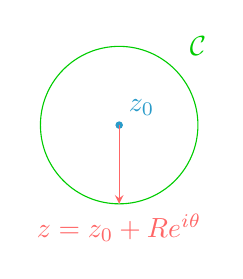
\begin{tikzpicture}[scale=2]
		\filldraw[cyan!80!black] (0, 0) circle (0.02) node [above right] {\( z_0 \)};
		\draw[green!80!black] (0, 0) circle (0.5);
		\node[green!80!black] at (0.5, 0.5) {\( \mathcal{C} \)};
		\draw[red!60!white, -stealth] (0, 0) -- (270:0.5) node[below] {\( z = z_0 + Re^{i \theta} \)};
	\end{tikzpicture}
\end{center}
then we write \( z = z_0 + Re^{i \theta} \), so we re-express \( z - z_0 = Re^{i \theta} \) in the definition
for \( f \). This definition also means \( dz = d\left( Re^{i \theta} \right) =
i Re^{i \theta} \diff \theta \). So, the contour integral becomes:
\begin{align*}
	\oint_{\mathcal{C}}f \diff z &= \int_{0}^{2\pi} \left( \sum_{n = -\infty}^{\infty} a_n (Re^{i \theta})^{n}
	\right) i Re^{i \theta} \diff \theta\\
	&= \sum_{n = -\infty}^{\infty} i \int_{0}^{2\pi}R^{n + 1} a_n e^{i (n + 1) \theta}\diff \theta \\ 
	&= \sum_{n = -\infty}^{\infty} i R^{n + 1}a_n \int_{0}^{2\pi} e^{i(n + 1) \theta}\diff \theta 
\end{align*}
Now, the integral over \( \theta \) is only nonzero when \( n = -1 \), where we have \( \int_{0}^{2\pi} \diff
\theta = 2\pi\). Therefore, the integral becomes:
\[
	\oint_{\mathcal{C}} f \diff z = 2 \pi i a_{-1}
\]
This quantity is sometimes called the \textbf{residue} of \( f \) at the point \( z_0 \), which is sometimes
denoted as \( \Res[f(z_0)] \). As an aside note, in the case where \( a_m  = 0 \) for all \( m \leq -2 \),
then we can find the residue \( a_{-1} \) by using:
\[
	\Res[f(z_0)] = a_{-1} = \lim_{z \to z_0} (z - z_0) f(z)
\]
This is true because if all the terms \( m \leq -2 \) are zero, then the only factor that doesn't contain a
\( z - z_0 \) term is \( a_{-1} \), so taking the limit immediately extracts the term. 
 
 
 


